\documentclass[crop,tikz,convert={outext=.svg,command=\unexpanded{pdf2svg \infile\space\outfile}},multi=false]{standalone}[2012/04/13]
%\usetikzlibrary{...}% tikz package already loaded by 'tikz' option
\makeatletter
\begin{document}
	% Created by tikzDevice version 0.12.3 on 2019-09-06 13:59:20
	% !TEX encoding = UTF-8 Unicode
	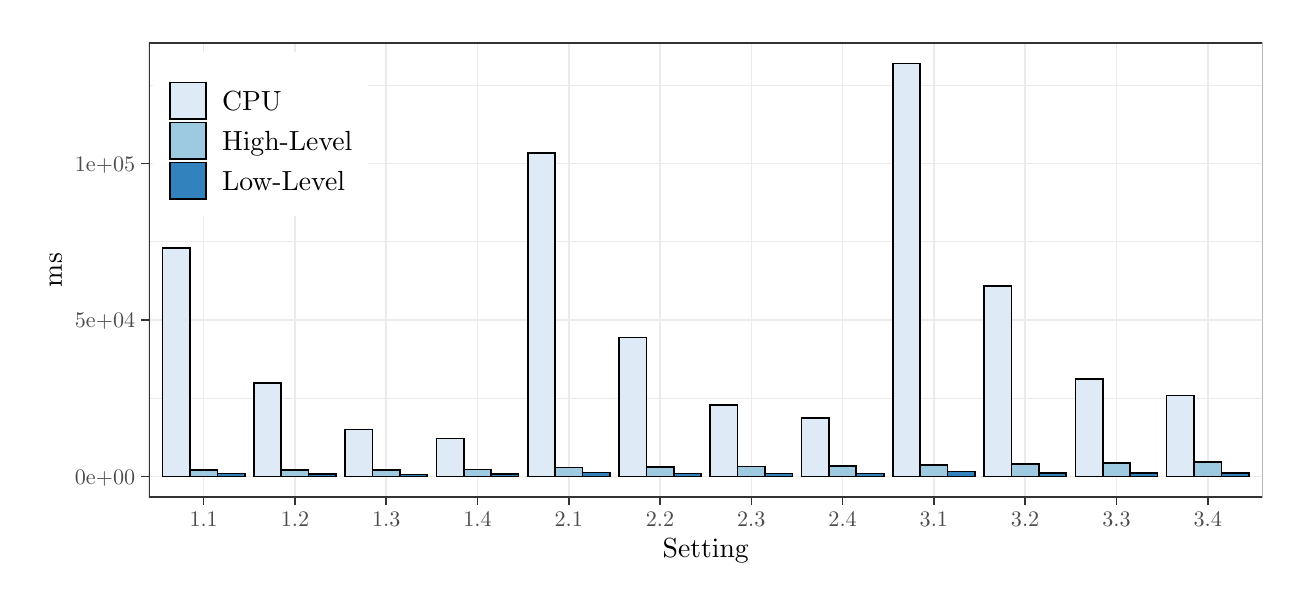
\begin{tikzpicture}[x=1pt,y=1pt]
	\definecolor{fillColor}{RGB}{255,255,255}
	\path[use as bounding box,fill=fillColor,fill opacity=0.00] (0,0) rectangle (451.69,198.74);
	\begin{scope}
	\path[clip] (  0.00,  0.00) rectangle (451.69,198.74);
	\definecolor{drawColor}{RGB}{255,255,255}
	\definecolor{fillColor}{RGB}{255,255,255}
	
	\path[draw=drawColor,line width= 0.6pt,line join=round,line cap=round,fill=fillColor] (  0.00,  0.00) rectangle (451.69,198.74);
	\end{scope}
	\begin{scope}
	\path[clip] ( 43.80, 29.10) rectangle (446.19,193.24);
	\definecolor{fillColor}{RGB}{255,255,255}
	
	\path[fill=fillColor] ( 43.80, 29.10) rectangle (446.19,193.24);
	\definecolor{drawColor}{gray}{0.92}
	
	\path[draw=drawColor,line width= 0.3pt,line join=round] ( 43.80, 64.83) --
	(446.19, 64.83);
	
	\path[draw=drawColor,line width= 0.3pt,line join=round] ( 43.80,121.38) --
	(446.19,121.38);
	
	\path[draw=drawColor,line width= 0.3pt,line join=round] ( 43.80,177.93) --
	(446.19,177.93);
	
	\path[draw=drawColor,line width= 0.6pt,line join=round] ( 43.80, 36.56) --
	(446.19, 36.56);
	
	\path[draw=drawColor,line width= 0.6pt,line join=round] ( 43.80, 93.11) --
	(446.19, 93.11);
	
	\path[draw=drawColor,line width= 0.6pt,line join=round] ( 43.80,149.66) --
	(446.19,149.66);
	
	\path[draw=drawColor,line width= 0.6pt,line join=round] ( 63.59, 29.10) --
	( 63.59,193.24);
	
	\path[draw=drawColor,line width= 0.6pt,line join=round] ( 96.58, 29.10) --
	( 96.58,193.24);
	
	\path[draw=drawColor,line width= 0.6pt,line join=round] (129.56, 29.10) --
	(129.56,193.24);
	
	\path[draw=drawColor,line width= 0.6pt,line join=round] (162.54, 29.10) --
	(162.54,193.24);
	
	\path[draw=drawColor,line width= 0.6pt,line join=round] (195.52, 29.10) --
	(195.52,193.24);
	
	\path[draw=drawColor,line width= 0.6pt,line join=round] (228.50, 29.10) --
	(228.50,193.24);
	
	\path[draw=drawColor,line width= 0.6pt,line join=round] (261.49, 29.10) --
	(261.49,193.24);
	
	\path[draw=drawColor,line width= 0.6pt,line join=round] (294.47, 29.10) --
	(294.47,193.24);
	
	\path[draw=drawColor,line width= 0.6pt,line join=round] (327.45, 29.10) --
	(327.45,193.24);
	
	\path[draw=drawColor,line width= 0.6pt,line join=round] (360.43, 29.10) --
	(360.43,193.24);
	
	\path[draw=drawColor,line width= 0.6pt,line join=round] (393.42, 29.10) --
	(393.42,193.24);
	
	\path[draw=drawColor,line width= 0.6pt,line join=round] (426.40, 29.10) --
	(426.40,193.24);
	\definecolor{drawColor}{RGB}{0,0,0}
	\definecolor{fillColor}{RGB}{49,130,189}
	
	\path[draw=drawColor,line width= 0.6pt,line cap=rect,fill=fillColor] ( 68.54, 36.56) rectangle ( 78.44, 37.58);
	\definecolor{fillColor}{RGB}{158,202,225}
	
	\path[draw=drawColor,line width= 0.6pt,line cap=rect,fill=fillColor] ( 58.65, 36.56) rectangle ( 68.54, 38.80);
	\definecolor{fillColor}{RGB}{222,235,247}
	
	\path[draw=drawColor,line width= 0.6pt,line cap=rect,fill=fillColor] ( 48.75, 36.56) rectangle ( 58.65,119.20);
	\definecolor{fillColor}{RGB}{49,130,189}
	
	\path[draw=drawColor,line width= 0.6pt,line cap=rect,fill=fillColor] (101.52, 36.56) rectangle (111.42, 37.36);
	\definecolor{fillColor}{RGB}{158,202,225}
	
	\path[draw=drawColor,line width= 0.6pt,line cap=rect,fill=fillColor] ( 91.63, 36.56) rectangle (101.52, 38.84);
	\definecolor{fillColor}{RGB}{222,235,247}
	
	\path[draw=drawColor,line width= 0.6pt,line cap=rect,fill=fillColor] ( 81.73, 36.56) rectangle ( 91.63, 70.37);
	\definecolor{fillColor}{RGB}{49,130,189}
	
	\path[draw=drawColor,line width= 0.6pt,line cap=rect,fill=fillColor] (134.50, 36.56) rectangle (144.40, 37.33);
	\definecolor{fillColor}{RGB}{158,202,225}
	
	\path[draw=drawColor,line width= 0.6pt,line cap=rect,fill=fillColor] (124.61, 36.56) rectangle (134.50, 38.99);
	\definecolor{fillColor}{RGB}{222,235,247}
	
	\path[draw=drawColor,line width= 0.6pt,line cap=rect,fill=fillColor] (114.72, 36.56) rectangle (124.61, 53.55);
	\definecolor{fillColor}{RGB}{49,130,189}
	
	\path[draw=drawColor,line width= 0.6pt,line cap=rect,fill=fillColor] (167.49, 36.56) rectangle (177.38, 37.36);
	\definecolor{fillColor}{RGB}{158,202,225}
	
	\path[draw=drawColor,line width= 0.6pt,line cap=rect,fill=fillColor] (157.59, 36.56) rectangle (167.49, 39.13);
	\definecolor{fillColor}{RGB}{222,235,247}
	
	\path[draw=drawColor,line width= 0.6pt,line cap=rect,fill=fillColor] (147.70, 36.56) rectangle (157.59, 50.31);
	\definecolor{fillColor}{RGB}{49,130,189}
	
	\path[draw=drawColor,line width= 0.6pt,line cap=rect,fill=fillColor] (200.47, 36.56) rectangle (210.36, 38.02);
	\definecolor{fillColor}{RGB}{158,202,225}
	
	\path[draw=drawColor,line width= 0.6pt,line cap=rect,fill=fillColor] (190.57, 36.56) rectangle (200.47, 39.84);
	\definecolor{fillColor}{RGB}{222,235,247}
	
	\path[draw=drawColor,line width= 0.6pt,line cap=rect,fill=fillColor] (180.68, 36.56) rectangle (190.57,153.47);
	\definecolor{fillColor}{RGB}{49,130,189}
	
	\path[draw=drawColor,line width= 0.6pt,line cap=rect,fill=fillColor] (233.45, 36.56) rectangle (243.35, 37.63);
	\definecolor{fillColor}{RGB}{158,202,225}
	
	\path[draw=drawColor,line width= 0.6pt,line cap=rect,fill=fillColor] (223.56, 36.56) rectangle (233.45, 39.96);
	\definecolor{fillColor}{RGB}{222,235,247}
	
	\path[draw=drawColor,line width= 0.6pt,line cap=rect,fill=fillColor] (213.66, 36.56) rectangle (223.56, 86.83);
	\definecolor{fillColor}{RGB}{49,130,189}
	
	\path[draw=drawColor,line width= 0.6pt,line cap=rect,fill=fillColor] (266.43, 36.56) rectangle (276.33, 37.60);
	\definecolor{fillColor}{RGB}{158,202,225}
	
	\path[draw=drawColor,line width= 0.6pt,line cap=rect,fill=fillColor] (256.54, 36.56) rectangle (266.43, 40.17);
	\definecolor{fillColor}{RGB}{222,235,247}
	
	\path[draw=drawColor,line width= 0.6pt,line cap=rect,fill=fillColor] (246.64, 36.56) rectangle (256.54, 62.34);
	\definecolor{fillColor}{RGB}{49,130,189}
	
	\path[draw=drawColor,line width= 0.6pt,line cap=rect,fill=fillColor] (299.42, 36.56) rectangle (309.31, 37.62);
	\definecolor{fillColor}{RGB}{158,202,225}
	
	\path[draw=drawColor,line width= 0.6pt,line cap=rect,fill=fillColor] (289.52, 36.56) rectangle (299.42, 40.41);
	\definecolor{fillColor}{RGB}{222,235,247}
	
	\path[draw=drawColor,line width= 0.6pt,line cap=rect,fill=fillColor] (279.63, 36.56) rectangle (289.52, 57.74);
	\definecolor{fillColor}{RGB}{49,130,189}
	
	\path[draw=drawColor,line width= 0.6pt,line cap=rect,fill=fillColor] (332.40, 36.56) rectangle (342.29, 38.40);
	\definecolor{fillColor}{RGB}{158,202,225}
	
	\path[draw=drawColor,line width= 0.6pt,line cap=rect,fill=fillColor] (322.50, 36.56) rectangle (332.40, 40.81);
	\definecolor{fillColor}{RGB}{222,235,247}
	
	\path[draw=drawColor,line width= 0.6pt,line cap=rect,fill=fillColor] (312.61, 36.56) rectangle (322.50,185.78);
	\definecolor{fillColor}{RGB}{49,130,189}
	
	\path[draw=drawColor,line width= 0.6pt,line cap=rect,fill=fillColor] (365.38, 36.56) rectangle (375.28, 37.91);
	\definecolor{fillColor}{RGB}{158,202,225}
	
	\path[draw=drawColor,line width= 0.6pt,line cap=rect,fill=fillColor] (355.49, 36.56) rectangle (365.38, 41.06);
	\definecolor{fillColor}{RGB}{222,235,247}
	
	\path[draw=drawColor,line width= 0.6pt,line cap=rect,fill=fillColor] (345.59, 36.56) rectangle (355.49,105.50);
	\definecolor{fillColor}{RGB}{49,130,189}
	
	\path[draw=drawColor,line width= 0.6pt,line cap=rect,fill=fillColor] (398.36, 36.56) rectangle (408.26, 37.88);
	\definecolor{fillColor}{RGB}{158,202,225}
	
	\path[draw=drawColor,line width= 0.6pt,line cap=rect,fill=fillColor] (388.47, 36.56) rectangle (398.36, 41.37);
	\definecolor{fillColor}{RGB}{222,235,247}
	
	\path[draw=drawColor,line width= 0.6pt,line cap=rect,fill=fillColor] (378.57, 36.56) rectangle (388.47, 71.78);
	\definecolor{fillColor}{RGB}{49,130,189}
	
	\path[draw=drawColor,line width= 0.6pt,line cap=rect,fill=fillColor] (431.35, 36.56) rectangle (441.24, 37.91);
	\definecolor{fillColor}{RGB}{158,202,225}
	
	\path[draw=drawColor,line width= 0.6pt,line cap=rect,fill=fillColor] (421.45, 36.56) rectangle (431.35, 41.68);
	\definecolor{fillColor}{RGB}{222,235,247}
	
	\path[draw=drawColor,line width= 0.6pt,line cap=rect,fill=fillColor] (411.56, 36.56) rectangle (421.45, 65.81);
	\definecolor{drawColor}{gray}{0.20}
	
	\path[draw=drawColor,line width= 0.6pt,line join=round,line cap=round] ( 43.80, 29.10) rectangle (446.19,193.24);
	\end{scope}
	\begin{scope}
	\path[clip] (  0.00,  0.00) rectangle (451.69,198.74);
	\definecolor{drawColor}{gray}{0.30}
	
	\node[text=drawColor,anchor=base east,inner sep=0pt, outer sep=0pt, scale=  0.80] at ( 38.85, 33.80) {0e+00};
	
	\node[text=drawColor,anchor=base east,inner sep=0pt, outer sep=0pt, scale=  0.80] at ( 38.85, 90.35) {5e+04};
	
	\node[text=drawColor,anchor=base east,inner sep=0pt, outer sep=0pt, scale=  0.80] at ( 38.85,146.90) {1e+05};
	\end{scope}
	\begin{scope}
	\path[clip] (  0.00,  0.00) rectangle (451.69,198.74);
	\definecolor{drawColor}{gray}{0.20}
	
	\path[draw=drawColor,line width= 0.6pt,line join=round] ( 41.05, 36.56) --
	( 43.80, 36.56);
	
	\path[draw=drawColor,line width= 0.6pt,line join=round] ( 41.05, 93.11) --
	( 43.80, 93.11);
	
	\path[draw=drawColor,line width= 0.6pt,line join=round] ( 41.05,149.66) --
	( 43.80,149.66);
	\end{scope}
	\begin{scope}
	\path[clip] (  0.00,  0.00) rectangle (451.69,198.74);
	\definecolor{drawColor}{gray}{0.20}
	
	\path[draw=drawColor,line width= 0.6pt,line join=round] ( 63.59, 26.35) --
	( 63.59, 29.10);
	
	\path[draw=drawColor,line width= 0.6pt,line join=round] ( 96.58, 26.35) --
	( 96.58, 29.10);
	
	\path[draw=drawColor,line width= 0.6pt,line join=round] (129.56, 26.35) --
	(129.56, 29.10);
	
	\path[draw=drawColor,line width= 0.6pt,line join=round] (162.54, 26.35) --
	(162.54, 29.10);
	
	\path[draw=drawColor,line width= 0.6pt,line join=round] (195.52, 26.35) --
	(195.52, 29.10);
	
	\path[draw=drawColor,line width= 0.6pt,line join=round] (228.50, 26.35) --
	(228.50, 29.10);
	
	\path[draw=drawColor,line width= 0.6pt,line join=round] (261.49, 26.35) --
	(261.49, 29.10);
	
	\path[draw=drawColor,line width= 0.6pt,line join=round] (294.47, 26.35) --
	(294.47, 29.10);
	
	\path[draw=drawColor,line width= 0.6pt,line join=round] (327.45, 26.35) --
	(327.45, 29.10);
	
	\path[draw=drawColor,line width= 0.6pt,line join=round] (360.43, 26.35) --
	(360.43, 29.10);
	
	\path[draw=drawColor,line width= 0.6pt,line join=round] (393.42, 26.35) --
	(393.42, 29.10);
	
	\path[draw=drawColor,line width= 0.6pt,line join=round] (426.40, 26.35) --
	(426.40, 29.10);
	\end{scope}
	\begin{scope}
	\path[clip] (  0.00,  0.00) rectangle (451.69,198.74);
	\definecolor{drawColor}{gray}{0.30}
	
	\node[text=drawColor,anchor=base,inner sep=0pt, outer sep=0pt, scale=  0.80] at ( 63.59, 18.64) {1.1};
	
	\node[text=drawColor,anchor=base,inner sep=0pt, outer sep=0pt, scale=  0.80] at ( 96.58, 18.64) {1.2};
	
	\node[text=drawColor,anchor=base,inner sep=0pt, outer sep=0pt, scale=  0.80] at (129.56, 18.64) {1.3};
	
	\node[text=drawColor,anchor=base,inner sep=0pt, outer sep=0pt, scale=  0.80] at (162.54, 18.64) {1.4};
	
	\node[text=drawColor,anchor=base,inner sep=0pt, outer sep=0pt, scale=  0.80] at (195.52, 18.64) {2.1};
	
	\node[text=drawColor,anchor=base,inner sep=0pt, outer sep=0pt, scale=  0.80] at (228.50, 18.64) {2.2};
	
	\node[text=drawColor,anchor=base,inner sep=0pt, outer sep=0pt, scale=  0.80] at (261.49, 18.64) {2.3};
	
	\node[text=drawColor,anchor=base,inner sep=0pt, outer sep=0pt, scale=  0.80] at (294.47, 18.64) {2.4};
	
	\node[text=drawColor,anchor=base,inner sep=0pt, outer sep=0pt, scale=  0.80] at (327.45, 18.64) {3.1};
	
	\node[text=drawColor,anchor=base,inner sep=0pt, outer sep=0pt, scale=  0.80] at (360.43, 18.64) {3.2};
	
	\node[text=drawColor,anchor=base,inner sep=0pt, outer sep=0pt, scale=  0.80] at (393.42, 18.64) {3.3};
	
	\node[text=drawColor,anchor=base,inner sep=0pt, outer sep=0pt, scale=  0.80] at (426.40, 18.64) {3.4};
	\end{scope}
	\begin{scope}
	\path[clip] (  0.00,  0.00) rectangle (451.69,198.74);
	\definecolor{drawColor}{RGB}{0,0,0}
	
	\node[text=drawColor,anchor=base,inner sep=0pt, outer sep=0pt, scale=  1.00] at (245.00,  7.44) {Setting};
	\end{scope}
	\begin{scope}
	\path[clip] (  0.00,  0.00) rectangle (451.69,198.74);
	\definecolor{drawColor}{RGB}{0,0,0}
	
	\node[text=drawColor,rotate= 90.00,anchor=base,inner sep=0pt, outer sep=0pt, scale=  1.00] at ( 12.39,111.17) {ms};
	\end{scope}
	\begin{scope}
	\path[clip] (  0.00,  0.00) rectangle (451.69,198.74);
	\definecolor{fillColor}{RGB}{255,255,255}
	
	\path[fill=fillColor] ( 45.28,130.73) rectangle (122.81,190.09);
	\end{scope}
	\begin{scope}
	\path[clip] (  0.00,  0.00) rectangle (451.69,198.74);
	\definecolor{fillColor}{RGB}{255,255,255}
	
	\path[fill=fillColor] ( 50.78,165.14) rectangle ( 65.23,179.59);
	\end{scope}
	\begin{scope}
	\path[clip] (  0.00,  0.00) rectangle (451.69,198.74);
	\definecolor{drawColor}{RGB}{0,0,0}
	\definecolor{fillColor}{RGB}{222,235,247}
	
	\path[draw=drawColor,line width= 0.6pt,line cap=rect,fill=fillColor] ( 51.49,165.85) rectangle ( 64.52,178.88);
	\end{scope}
	\begin{scope}
	\path[clip] (  0.00,  0.00) rectangle (451.69,198.74);
	\definecolor{fillColor}{RGB}{255,255,255}
	
	\path[fill=fillColor] ( 50.78,150.69) rectangle ( 65.23,165.14);
	\end{scope}
	\begin{scope}
	\path[clip] (  0.00,  0.00) rectangle (451.69,198.74);
	\definecolor{drawColor}{RGB}{0,0,0}
	\definecolor{fillColor}{RGB}{158,202,225}
	
	\path[draw=drawColor,line width= 0.6pt,line cap=rect,fill=fillColor] ( 51.49,151.40) rectangle ( 64.52,164.43);
	\end{scope}
	\begin{scope}
	\path[clip] (  0.00,  0.00) rectangle (451.69,198.74);
	\definecolor{fillColor}{RGB}{255,255,255}
	
	\path[fill=fillColor] ( 50.78,136.23) rectangle ( 65.23,150.69);
	\end{scope}
	\begin{scope}
	\path[clip] (  0.00,  0.00) rectangle (451.69,198.74);
	\definecolor{drawColor}{RGB}{0,0,0}
	\definecolor{fillColor}{RGB}{49,130,189}
	
	\path[draw=drawColor,line width= 0.6pt,line cap=rect,fill=fillColor] ( 51.49,136.94) rectangle ( 64.52,149.97);
	\end{scope}
	\begin{scope}
	\path[clip] (  0.00,  0.00) rectangle (451.69,198.74);
	\definecolor{drawColor}{RGB}{0,0,0}
	
	\node[text=drawColor,anchor=base west,inner sep=0pt, outer sep=0pt, scale=  1.00] at ( 70.23,168.92) {CPU};
	\end{scope}
	\begin{scope}
	\path[clip] (  0.00,  0.00) rectangle (451.69,198.74);
	\definecolor{drawColor}{RGB}{0,0,0}
	
	\node[text=drawColor,anchor=base west,inner sep=0pt, outer sep=0pt, scale=  1.00] at ( 70.23,154.47) {High-Level};
	\end{scope}
	\begin{scope}
	\path[clip] (  0.00,  0.00) rectangle (451.69,198.74);
	\definecolor{drawColor}{RGB}{0,0,0}
	
	\node[text=drawColor,anchor=base west,inner sep=0pt, outer sep=0pt, scale=  1.00] at ( 70.23,140.02) {Low-Level};
	\end{scope}
	\end{tikzpicture}
\end{document}